\documentclass[10pt,letterpaper]{article}
\usepackage[margin=1in]{geometry}
\usepackage[T1]{fontenc}
\usepackage{lmodern,microtype,amsmath,amssymb,amsthm,booktabs,array,graphicx,xurl}
\usepackage[hidelinks]{hyperref}
\usepackage{enumitem,placeins}
\microtypesetup{protrusion=false}
\setlist{nosep,leftmargin=*}
\setlength{\parskip}{3pt}
\setlength{\parindent}{1em}
\newtheorem{theorem}{Theorem}
\newtheorem{lemma}[theorem]{Lemma}
\newtheorem{proposition}[theorem]{Proposition}
\newtheorem{corollary}[theorem]{Corollary}
\newcommand{\ind}{\mathbf 1}
\newcommand{\R}{\mathbb R}
\newcommand{\dist}{\operatorname{dist}}
\newcommand{\D}{\mathcal D}
\newcommand{\F}{\mathcal F}
\title{GeoCert: Certified Expression Intervals under Segmentation Uncertainty in Spatial Transcriptomics}
\author{Arnav Peram\\[3pt]\normalsize Arizona College Preparatory High School\\\normalsize\texttt{arnavperam1@gmail.com}}
\date{}
\renewcommand{\abstractname}{\normalsize Abstract}
\begin{document}
\hypersetup{pdftitle={GeoCert: Certified Expression Intervals under Segmentation Uncertainty in Spatial Transcriptomics},pdfauthor={Arnav Peram},pageanchor=false}
\begin{titlepage}\maketitle\thispagestyle{empty}
\begin{abstract}\normalsize
A shared cell-boundary error can alter several expression counts together in imaging-based spatial transcriptomics. We introduce GeoCert, an exact method for determining which observed cell-by-gene counts remain invariant under a physical boundary-deformation budget and which can change. We show that, for ordered boundaries subject to slope, band, thickness and nuclear constraints, the minimum summed interface displacement for every feasible molecular assignment can be encoded in a single polynomial-size graph with rational capacities. For point transcripts along one interface, we use exact critical heights in a count dynamic program that computes hard-budget optima in polynomial time, even when penalized cuts leave a gap. For disjoint two-label ribbons, an exact coordinate conversion gives physical changed-label area; gluing and min-plus composition then enforce one compatible tissue partition and a shared area budget. We also allow different ribbon widths through a union of complete atlases that preserves every deformation permitted by the primary atlas. On Xenium lung crops and a breast format-test dataset, five atlas families per crop yield 496,604 exact interval rows over 17 budgets. At 4 \textmu m\texttwosuperior{}, their union widens 298 lung and 3,595 breast intervals relative to the primary atlas. Across the budget grid, shared geometry tightens independent-molecule outer bounds for 29 of 102 lung and 791 of 2,076 breast cell--gene pairs whose outer interval reaches a width of at least two. The same effect appears in two breast cancer donors: under the primary atlas, shared geometry tightens independent-molecule bounds for 13.8\% and 11.7\% of eligible cell--gene pairs. For each interval endpoint, we provide a boundary that shows how the reported count is attained and when multiple molecular transfers share one deformation.
\end{abstract}
\end{titlepage}
\hypersetup{pageanchor=true}\setcounter{page}{1}

\begin{figure}[t]\centering
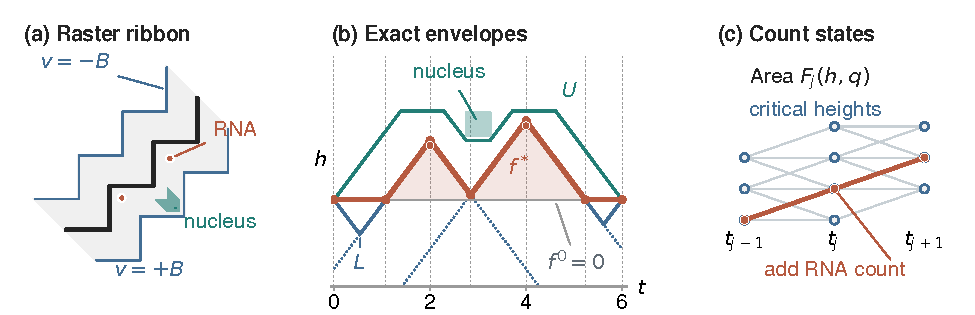
\includegraphics[width=\textwidth]{figures/geometry_pipeline.pdf}
\caption{From a shared boundary to an exact count spectrum (schematic): (a) a ribbon follows the raster interface; (b) a shear chart straightens it, and molecular requirements define Lipschitz envelopes whose clamp of the reference minimizes area; and (c) critical heights give a count-indexed path computation. Theorem~\ref{thm:glue} converts chart displacement to physical area and glues local witnesses.}\label{fig:geometry}
\end{figure}

\section{Introduction}
In imaging-based spatial transcriptomics, cell boundaries determine which molecules contribute to each expression count~\cite{baysor,proseg}. Consider a breast format-test cell with 22 LDHB molecules: treating transfers independently allows a count of 17 at a $0.25\,\mu\mathrm m^2$ area budget, whereas the smallest count attainable under the same boundary rules is 19 (Figure~\ref{fig:witness}). The five removals cost too much together. For low-count markers, such dependencies can determine whether a cell remains positive.

GeoCert finds the smallest and largest counts within a specified boundary family (Figure~\ref{fig:geometry}). An \emph{atlas} collects disjoint boundary regions, called \emph{ribbons}, whose allowed movements form one compatible tissue partition. The \emph{budget} limits the total area that changes cell label; a \emph{witness} is a partition that attains a reported count. Equal endpoints certify invariance within this family. We measure \emph{reach} as the fraction of individual count changes from another segmentation that the family can reproduce.

\paragraph{Related work.}
Baysor, Proseg, BIDCell and Segger estimate segmentations or transcript assignments~\cite{baysor,proseg,bidcell,segger}, whereas ResolVI models downstream misassignment probabilistically~\cite{resolvi} and TISSUE gives uncertainty intervals for predicted, unmeasured expression~\cite{tissue}. Related diagnostics include ovrlpy's analysis of three-dimensional signal overlap~\cite{ovrlpy}. GeoCert complements these approaches by computing how counts of already observed molecules can change under geometric alternatives to a reference segmentation.

The construction draws on convex segmentation and ordered-label cuts~\cite{hochbaum,ishikawa}, interacting-surface graphs~\cite{li,shah}, higher-order energies~\cite{kz,kohli}, Lipschitz extensions~\cite{mcshane,whitney}, and difference-potential lattices~\cite{felsner}. Although submodularity alone does not guarantee a binary graph representation with auxiliaries~\cite{zivny}, we establish such a representation for the continuous assignment cost. Alongside this cut formulation, exact critical heights support resource-state dynamic programming~\cite{joksch} for hard budgets.



Our contributions are:
\begin{itemize}
\item \textbf{Exact deformation costs.} One polynomial-size rational graph represents the minimum displacement for every feasible assignment and supports arbitrary unary costs (Theorem~\ref{thm:cost}; coupled interfaces in Supplement~\S1).
\item \textbf{Exact counts under hard budgets.} For point transcripts along one interface, a polynomial-time dynamic program finds count optima that penalized cuts can miss (Theorem~\ref{thm:chain}).
\item \textbf{Tissue-wide witnesses.} Disjoint ribbons combine into a topology-preserving partition under one area budget, with checkable endpoint witnesses. A union of complete atlases permits alternative widths while retaining the primary family (Theorem~\ref{thm:glue}, Proposition~\ref{thm:union}).
\end{itemize}

\section{Exact elimination of continuous boundary costs}\label{sec:engine}
We first fix the proposed transcript assignments and find the least boundary displacement needed to realize them. The assignments impose upper and lower requirements; their propagated envelopes determine feasibility and minimum displacement. We prove this for one moving interface. Supplement~\S1 extends the construction to ordered interfaces with heterogeneous slopes and minimum/maximum thickness constraints.

\subsection{Requirements and feasible assignments}
Let $f:I\to\mathbb R$ be an $s$-Lipschitz boundary on a compact rational interval, with band $[\underline b,\overline b]$ and fixed endpoints, and let $f^0$ be a rational piecewise-affine reference satisfying the same constraints. To specify ownership on either side, we represent site $i$ by a rectangle $[x_i^-,x_i^+]\times I_i$, allowing degenerate points. Sites in group $g(i)$ share owner $c_g\in\{0,1\}$, encoded by $b_g=\ind[c_g=0]$, so clearance $\rho>0$ requires
\begin{equation}
 b_{g(i)}=1\Rightarrow f(t)\ge\ell_i=x_i^++\rho,\qquad
 b_{g(i)}=0\Rightarrow f(t)\le u_i=x_i^--\rho\quad(t\in I_i).\label{eq:owners}
\end{equation}
Nuclear regions are fixed-label groups with the same geometric requirements and zero molecular reward. The reference satisfies the geometry but may violate uncertain-site assignment requirements.

\begin{lemma}[Propagation on one interface]\label{lem:kernel}
A lower interval requirement $f\ge\ell_i$ on $I_i$ implies
$f(t)\ge\ell_i-s\dist(t,I_i)$ everywhere. An upper requirement analogously implies $f(t)\le u_i+s\dist(t,I_i)$.
\end{lemma}
\begin{proof}
The Lipschitz inequality between $t$ and its closest point in the closed interval $I_i$ gives both bounds. Without further restrictions, the corresponding tent profiles attain them.
\end{proof}

We forbid a lower activation when $\ell_i>\overline b$ or $\ell_i>f^0(e)+s\dist(e,I_i)$ at either endpoint $e$, and an upper activation when $u_i<\underline b$ or $f^0(e)>u_i+s\dist(e,I_i)$. Along with structural pins, we impose $b_{g(i)}\Rightarrow b_{g(j)}$ whenever $\ell_i-s\dist(I_i,I_j)>u_j$, excluding incompatible lower and upper requirements.

\begin{theorem}[Exact assignment feasibility]\label{thm:feas}
The finite unary restrictions, implications and structural pins characterize the assignments realizable by the continuous family.
\end{theorem}
\begin{proof}
Necessity follows from Lemma~\ref{lem:kernel}. For sufficiency, let $L$ be the maximum of the active lower tents, lower band and endpoint lower cones, and $U$ the corresponding minimum for upper requirements. Since $\dist(t,I_i)+\dist(t,I_j)\ge\dist(I_i,I_j)$, the pair tests place every lower contribution below every upper contribution. Unary tests handle bands and endpoints, so $L\le U$. Both envelopes are $s$-Lipschitz and satisfy the bands, endpoint equalities and selected requirements, giving continuous feasible boundaries.
\end{proof}

\subsection{Preserving every assignment's minimum displacement}
For complete owners $c$, write $\mathcal F(c)$ for the realizing boundaries and
\begin{equation}
 D^\star(c)=\min_{f\in\mathcal F(c)}\int_I|f-f^0|\,dt,\qquad \min\varnothing=+\infty.\label{eq:dstar}
\end{equation}
The minimum $D^\star(c)$, converted to physical area in Section~\ref{sec:atlas}, is generally nonadditive across transcripts because one boundary movement can transfer several molecules.

\begin{theorem}[Assignment-wise cost representation]\label{thm:cost}
For rational input, one polynomial-size rational graph with assignment vertices $b(c)$, auxiliary vertices $y$, logical hard arcs and a known constant $\kappa$ satisfies
\begin{equation}
\min_y\operatorname{Cut}_{G_D}(b(c),y)+\kappa=D^\star(c)\label{eq:identity}
\end{equation}
for every feasible assignment. Hard-feasible cuts exist exactly for realizable assignments. After adding arbitrary rational unary molecular costs and a rational $\lambda\ge0$, a minimum cut detects infeasibility or returns optimal owners and an attaining rational piecewise-affine boundary.
\end{theorem}
\begin{proof}
Scalar minimum and maximum preserve the slope, band and endpoint constraints. Consequently
\begin{equation}
f^*(t)=\min\{U(t),\max\{L(t),f^0(t)\}\}\label{eq:clamp}
\end{equation}
is feasible. Every realization lies between $L$ and $U$, so this clamp is pointwise nearest to $f^0$ and minimizes its integrated displacement.

The positive displacement is the maximum of activated functions $[\ell_i-s\dist(t,I_i)-f^0(t)]_+$; negative displacement uses upper requirements and complementary bits. In forming these envelopes, we retain all fixed and uncertain-site requirements, including source-inconsistent ones. For feasible owners, these displacements cannot occur at the same point, so we integrate them separately. To integrate each piecewise-affine envelope, we partition at piece endpoints, source knots, zeros and pair crossings. Positive heights then have fixed order $h_1\ge\cdots\ge h_k>0$ on each slab, with $h_{k+1}=0$. If $S_j$ contains the first $j$ activation labels, then
\begin{equation}
\max_{i\ \mathrm{active}}h_i=\sum_{j=1}^k(h_j-h_{j+1})\ind[S_j\hbox{ has an active label}].\label{eq:layers}
\end{equation}
Integrating the nonnegative affine differences gives exact weights for standard OR helpers~\cite{kz,kohli}, with the construction reversed for complementary polarity. Repeated group labels share one bit; mandatory terms use forced helpers or $\kappa$. Minimizing auxiliaries therefore recovers the integrated clamp for each fixed $b(c)$, proving~\eqref{eq:identity} before molecular costs are chosen. We add unary costs by successive differences, recording a constant shift for negative terms, and scale rational capacities to integers. Each hard capacity exceeds the finite-capacity sum for the chosen costs and $\lambda$. An optimal cut through a hard arc certifies infeasibility; otherwise,~\eqref{eq:clamp} gives an attaining boundary.
\end{proof}

\paragraph{Complexity and coupled interfaces.}
With $M$ constant-piece excursion profiles, relative order changes $O(M^2)$ times. Each adjacent swap changes one prefix, so merging repeated helpers leaves $O(M^2+M)$ activation helpers. For $G$ groups and $N$ molecular/structural sites, the graph has $O(G+M^2+M)$ vertices and $O(G+N^2+M^2+M)$ arcs. Since intersections and integrated weights have polynomial rational encoding, an event sweep~\cite{bentley} can construct the graph in polynomial time, accumulating unchanged layer integrals lazily; Supplement~\S3 gives the full construction bound.

For coupled interfaces, we first propagate constraints along boundary-separation paths. The resulting envelopes are closed under componentwise minimum and maximum, making the clamp simultaneously feasible and preserving the identity for assignments of $m+1$ labels (Supplement~\S1). Its cost is summed interface displacement; the physical-area identity below uses disjoint two-label ribbons. For the scalar point-transcript atlas, Section~\ref{sec:counts} instead adds count states to the clamp's exact critical mesh and solves hard budgets directly.

\section{From local interfaces to one compatible tissue model}\label{sec:atlas}
Local count changes can be interpreted together only when their boundaries belong to one tissue partition. An \emph{atlas} consists of two-label ribbons around reference interfaces, with disjoint interiors, fixed endpoint traces and outer rails. The partition outside the ribbons stays fixed.

Let $P_i$ be closed ribbons with pairwise disjoint interiors and injective charts $\Psi_i:I_i\times[-B_i,B_i]\to P_i$. The reference boundary is transverse coordinate zero, each half lies wholly in its stated reference label, and each RNA belongs to at most one ribbon. An allowed displacement $h_i$ is continuous, zero at both endpoints, and $|h_i|\le qB_i$ for $q<1$. Fixed regions have additional label constraints.

\begin{samepage}
\begin{theorem}[Compatible gluing and additive physical area]\label{thm:glue}
Every tuple of admissible ribbon boundaries is induced by one global homeomorphism of the reference partition, identity outside the ribbon interiors. For constant chart Jacobians $J_i>0$, the physical area whose label changes is exactly $\sum_i J_i\int|h_i|$.
\end{theorem}
\end{samepage}
\begin{proof}
For fixed $t$, define a map of $[-B_i,B_i]$ by
\begin{equation}
H_i(t,v)=\begin{cases}
-B_i+(v+B_i)(h_i(t)+B_i)/B_i,&v\le0,\\
h_i(t)+v(B_i-h_i(t))/B_i,&v\ge0.
\end{cases}\label{eq:homeo}
\end{equation}
Both slopes are positive and bounded away from zero. The branches meet at $h_i(t)$, have continuous explicit inverses, and fix the rails; at interval endpoints the map is the identity. Conjugating $(t,v)\mapsto(t,H_i(t,v))$ by $\Psi_i$ therefore gives a homeomorphism fixing the ribbon boundary. We extend it by the identity outside the ribbon. These finitely many maps and their inverses agree on intersections, so they glue to a global homeomorphism preserving cell topology and fixed junction incidences. Within each ribbon, the changed-label region lies between zero and $h_i(t)$ and has chart area $\int|h_i|$. The area formula follows by change of variables and disjointness of the interiors.
\end{proof}

\paragraph{Exact chart for a raster interface.}
For a coordinate-monotone raster-edge path choose $s_x,s_y\in\{-1,1\}$ and let $t=s_xx+s_yy$, $u=s_xx-s_yy$ in pixel coordinates. The exact source arc is $u=r_i(t)$. With pixel size $p$,
\begin{equation}
\Psi_i(t,h)=\frac p2\big(s_x(t+r_i(t)+h),\ s_y(t-r_i(t)-h)\big),\qquad J_i=p^2/2,\label{eq:chart}
\end{equation}
up to the recorded origin. This shear preserves the staircase interface exactly and has constant Jacobian except at measure-zero corners, so we optimize displacement $h$ from the zero source in these coordinates. The admissible motion is further restricted by conservative interval constraints from intersecting nuclear pixels, preserving their owners, and by fixed junction neighborhoods and uncovered perimeter portions. These fixed regions allow arbitrary reference adjacency while defining the atlas's topology and coverage.



\section{Hard budgets without assignment enumeration}\label{sec:counts}
A penalized cut trades count against area, but some hard-budget optima are missed for every penalty (\S\ref{sec:penalties}). We therefore compute the least area needed for each count directly.
Here $D^\star$ includes the chart Jacobians from Theorem~\ref{thm:glue}. For a retained count $N_{kg}(c)$, define the minimum-area spectrum
\begin{equation}
S_{kg}(q)=\min_{c:N_{kg}(c)=q}D^\star(c),\quad
[L_{kg}(\delta),U_{kg}(\delta)]=\left[\min,\max\right]\{q:S_{kg}(q)\le\delta\}.\label{eq:interval}
\end{equation}
The endpoints are the smallest and largest feasible counts; intermediate integers need not all be feasible. We return an attaining boundary for each endpoint and report an empty feasible-count set separately.

\subsection{Exact critical heights and a count chain}
For point transcripts along one boundary, we collect all propagated lower/upper requirement pieces, fixed geometric pieces and source pieces before choosing owners. Their endpoints and crossings, including source crossings and every point observation, define a common mesh. At node $t_j$, candidate values $V_j$ lie within forced envelopes and satisfy every point's clearance gap and fixed constraints.

\begin{lemma}[Exact scalar critical mesh]\label{lem:mesh}
Restricting nodal heights to these candidates, enforcing original adjacent slope and ownership constraints, and charging trapezoidal absolute displacement preserves $D^\star(c)$ for every feasible assignment.
\end{lemma}
\begin{proof}
Between consecutive events, all candidate pieces are affine with fixed ordering. The clamp~\eqref{eq:clamp} follows one piece and has constant-sign displacement, so its retained nodal values have trapezoidal area equal to its exact integral. Conversely, any feasible candidate-height path interpolates to a feasible continuous boundary: the mesh contains every constraint endpoint, and constraints between them are linear. Its trapezoidal cost upper-bounds its absolute-displacement integral, which is at least $D^\star(c)$. Since the canonical minimizer is retained, equality is attained.
\end{proof}

\begin{samepage}
\begin{theorem}[Polynomial exact spectra for explicit point RNAs]\label{thm:chain}
Assume one boundary, one point per free RNA group, arbitrary fixed structural intervals, and a nonnegative integer per-point count score. Let $W$ be its variable range and $H_j=|V_j|$. Given the critical mesh and its local node scores, the count dynamic program uses $O((W+1)\sum_jH_j)$ arithmetic transition operations and returns every minimum-area count, with backpointers to attaining boundaries. With explicit unit transcripts the complete algorithm is polynomial in the input and rational encoding.
\end{theorem}
\end{samepage}
\begin{proof}
A permitted height at a point's mesh node determines its owner uniquely because we excluded the clearance gap. We count each observation once at its node. Let $z_j(h)$ be the local score and $a_j(h)=w_j|h-f^0(t_j)|$, where $w_j$ is half the sum of adjacent mesh lengths. The recurrence is
\begin{equation}
F_j(h,q)=a_j(h)+\min_{u\in V_{j-1}:|u-h|\le s(t_j-t_{j-1})}
F_{j-1}(u,q-z_j(h)).\label{eq:dp}
\end{equation}
We initialize with the fixed groups and first node. The usual shortest-path induction gives the exact nodal minimum for each count; Lemma~\ref{lem:mesh} identifies it with the continuous minimum, including outcomes missed by penalties. For each predecessor count, the allowed sorted predecessors form a sliding interval as $h$ increases. A monotone queue finds its minima in $O(H_{j-1}+H_j)$ operations. Summing over counts and nodes gives the runtime, and backpointers recover attaining boundaries.
For $P$ affine pieces, the full mesh has $O(P^2+P)$ nodes and $O(P)$ candidates per node. Rational intersection arithmetic therefore gives polynomial preparation and encoding. With unit RNA scores, $W$ is bounded by the explicit molecule count; binary-compressed multiplicities give pseudo-polynomial dependence. Free interval-valued RNA groups and arbitrary coupled height vectors require further state and fall outside this scalar result.
\end{proof}

Resource-state shortest paths are standard~\cite{joksch}; the critical-mesh lemma makes their costs exact for the continuous problem. Single-copy queries, however, need no count chain when the source satisfies every source-owner and structural constraint at zero cost: we propagate requested bits, retain unforced source bits, and reconstruct the clamp. This gives minimum area because every costly requirement is forced in all feasible completions, whereas the general theorem needs no such source-assignment assumption.

\subsection{One area allowance for the entire atlas}
For a fixed cell and gene, let $S_i(d)$ be the least physical area among all feasible states of patch $i$ with \emph{count change} $d$ from its source. Here $i=1,\ldots,r$ ranges over the complete atlas, including patches that cannot change this count. With $n^0_{kg}$ the reference count, including RNA outside ribbons,
\begin{equation}
S_{kg}(q)=\min_{d_1+\cdots+d_r=q-n^0_{kg}}\sum_{i=1}^r S_i(d_i).\label{eq:convolution}
\end{equation}
This min-plus convolution is exact in both directions. A minimizing trace selects one witness per patch, which Theorem~\ref{thm:glue} combines into a global partition. Conversely, every allowed partition decomposes into patch states costing at least their local minima. A patch without the target gene contributes only $S_i(0)$, its minimum required area. It can be omitted when its source assignment is feasible at zero cost; otherwise this cost and an attaining witness must be retained. An infeasible patch makes the atlas infeasible. Direct convolution takes $O(r(W+1)^2)$ operations. The tissue atlases satisfy the zero-cost source condition on every patch (Supplement~\S9.5).

Counting each molecule once and sharing budget $\delta$ across patches puts every allowed count matrix componentwise within the intervals. However, endpoints from different rows may require different partitions, so joint marker questions need vector spectra or a joint predicate instead of products of marginal endpoints.

\subsection{Alternative complete atlases}
Width-specific atlases can offer different feasible deformations. Their union preserves these alternatives without requiring their supports to be nested.

\begin{proposition}[Exact finite-family certificates]\label{thm:union}
Let $\mathcal F_1,\ldots,\mathcal F_A$ be complete atlas families with the same reference partition, counted observations and physical-area cost. If $S_a(q)$ is the exact count spectrum of member $a$, then the family $\mathcal F_\cup=\bigcup_{a=1}^A\mathcal F_a$ has spectrum
\begin{equation}
 S_\cup(q)=\min_a S_a(q).\label{eq:union}
\end{equation}
Every finite minimum inherits an attaining boundary and its member identity. At budget $\delta$, $L_\cup=\min_a L_a$ and $U_\cup=\max_a U_a$, omitting members with empty feasible-count sets; the union is empty exactly when all members are empty.
\end{proposition}
\begin{proof}
Each partition in the union belongs to a member and costs at least that member's minimum for its count. Conversely, a member attaining the least finite minimum supplies a partition in the union at that cost. Taking the extreme budget-feasible counts proves the endpoint identities.
\end{proof}
Taking the pointwise minimum costs $O(\sum_a|\operatorname{dom}S_a|)$ comparisons. Each witness retains one complete atlas and its compatible ribbons. Including the primary atlas preserves all its feasible states and every reference count it can attain on the same cell--gene pairs. Joint predicates likewise select a complete atlas; mixing patches from different atlases would define a different model.

\subsection{Limitations of Lagrangian penalties}\label{sec:penalties}
By weak duality, an exact cut yielding $m(\mu)=\min_c\{\mu D^\star(c)-N(c)\}$ gives
\begin{equation}
U(\delta)\le\left\lfloor\mu\delta-m(\mu)\right\rfloor,\qquad\mu\ge0.\label{eq:dual}
\end{equation}
Feasible witnesses give the opposite bound, leaving a gap unless exact refinement closes it. Applying the same argument to $-N$ bounds the lower endpoint.

To see why this bound can be loose, consider eight \emph{distinct, explicit unit} transcripts with source zero on $[0,30]$, slope one, band $[-4,4]$, and clearance $1/10$. We place clusters of $2,3,3$ RNAs at longitudinal centers $5,15,25$. In a cluster of height $a=2,3,3$, respectively, point $j$ is $(t,x)=(\mathrm{center}+j/100,a-j/100-1/10)$. Clearance forces common ownership within each cluster; its first cone dominates, and cluster supports are disjoint. The exact count/area states are $(0,0),(2,4),(3,9),(5,13),(6,18),(8,22)$. At budget ten the maximum is three, whereas the best penalty upper bound is four: for $\mu\le1/3$, the count-eight state gives $B(\mu)\ge8-12\mu\ge4$; for $\mu\ge1/3$, the count-two state gives $B(\mu)\ge2+6\mu\ge4$. Thus the best penalty bound is four at $\mu=1/3$, while the count chain recovers the true optimum of three using only explicit unit transcripts.

\section{Evaluation: count effects and geometric reach}\label{sec:eval}
The theory gives exact count intervals for a specified family of boundaries. We now ask when shared geometry changes the answer obtained by treating molecules independently, whether that effect recurs in biological donors, and how ribbon width limits the changes the model can represent.
\subsection{Data and atlas construction}
We apply the same extraction rule to two crops from one public Xenium lung specimen~\cite{data,xenium} and two breast format-test crops~\cite{breasttest} (Table~\ref{tab:scope}). Connected cells away from crop borders are retained and their interfaces split into monotone arcs. The primary atlas tries chart halfwidths $B=4,2,1,1/2$ in order, accepting disjoint ribbons with slope one, band $|h|\le3B/4$ and fixed nuclear owners (Supplement~\S2).

\begin{table}[!htbp]\centering
\begin{tabular}{lrr}\toprule
Quantity&Lung crops&Breast format-test crops\\\midrule
Retained Q20 RNA&7,370&81,182\\
Crop-contained connected cells&153&467\\
Disjoint ribbons&544&1,708\\
RNA inside ribbons&745&8,262\\
Editable incident-edge coverage&68.3\%&65.8\%\\
Cell--gene spectra&3,304&22,976\\
\bottomrule
\end{tabular}
\caption{Primary-atlas coverage includes cells without editable arcs. Spectra cover positive or editable cell--gene pairs and include fixed RNA outside ribbons.}\label{tab:scope}
\end{table}

\FloatBarrier
\subsection{Certified invariance and shared-boundary count changes}\label{sec:effects}
At a $4\,\mu\mathrm m^2$ area budget, 84.1\% of lung and 77.1\% of breast cell--gene counts are invariant within the primary atlas, whose maximum displacement is about $0.45\,\mu\mathrm m$ (\S\ref{sec:saturation}). These fractions include counts fixed outside editable ribbons. Supplement~\S6 gives all eight budgets from zero to $4\,\mu\mathrm m^2$.

There are two ways that treating molecules separately can distort these intervals. A marginal outer bound allows every individually affordable transfer, even when the transfers together exceed the budget or require incompatible boundaries. In the other direction, an additive inner approximation enforces feasibility but charges the sum of the individual transfer areas. It can overcharge when several molecules move with one boundary shift.

\begin{figure}[!htbp]\centering
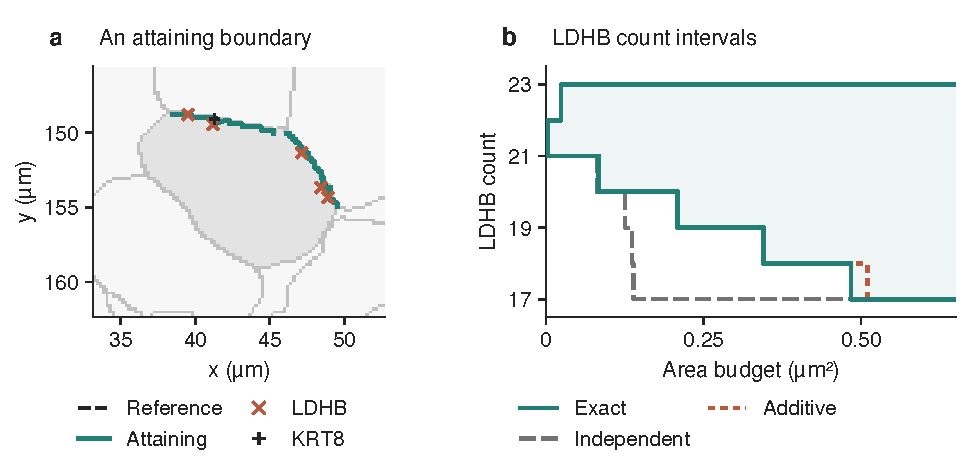
\includegraphics[width=\textwidth]{figures/ldhb_composite.pdf}
\caption{Shared geometry changes the LDHB interval in breast cell 81. (a) Two compatible boundary changes attain count 17; crosses mark five LDHB transfers and the plus marks collateral KRT8. (b) Exact interval endpoints and the independent-molecule outer and additive inner bounds. Steps occur at exact minimum areas; shading marks the exact interval.}\label{fig:witness}
\end{figure}

Breast cell 81 makes the distinction concrete (Figure~\ref{fig:witness}). Its reference LDHB count is 22. At $0.25\,\mu\mathrm m^2$, the marginal bound allows a count of 17, but the exact minimum is 19: five removals cost too much together. At $0.5\,\mu\mathrm m^2$, those removals become possible, while the additive approximation still allows only four. The witness moves three LDHB molecules through one ribbon and two through another, with one collateral KRT8 transfer. Both deformations fit within the shared budget, using about $0.48\,\mu\mathrm m^2$ in total.

We measure this dependence on cell--gene pairs whose marginal interval has width at least two somewhere on the original budget grid. Exact geometry tightens the bound for 4 of 46 lung pairs (8.7\%) and 203 of 1,026 breast pairs (19.8\%), affecting 4 of 153 lung cells and 139 of 467 breast cells. On the finer, 17-budget grid, these fractions rise to 26.1\% and 35.2\%, revealing differences between the original budget points (Supplement~\S7). The additive approximation also misses attainable endpoints (Supplement~\S6).

\paragraph{Joint marker co-detection.}
We also ask whether EPCAM and PTPRC remain detected in the same cell under a common deformation. At $0.25\,\mu\mathrm m^2$, five of seven initially co-detected lung cells and 46 of 48 breast cells retain both markers throughout the primary atlas family. For the other two cells in each dataset, a witness removes co-detection. These joint certificates persist through budget $4$ (Supplement~\S8.4), showing how the geometry can answer a multi-gene question.

\FloatBarrier
\subsection{Replication in breast cancer donors}\label{sec:donors}
We next tested the primary atlas on biological breast tissue, using three predefined $200\,\mu\mathrm m$ regions from each of two donors with ductal and lobular carcinoma~\cite{biologicalbreast}. Together, these regions contain 1,518 complete cells. We kept the atlas rules unchanged: ribbons cover about 76\% of eligible shared edges and allow at most $0.45\,\mu\mathrm m$ of displacement. Within this family, 79.6\% of ductal-sample counts and 83.5\% of lobular-sample counts are invariant at $4\,\mu\mathrm m^2$.

The shared-boundary effect recurs in all six regions (Figure~\ref{fig:donors}a). Pooled within donor, exact geometry tightens 13.8\% of eligible ductal-sample pairs and 11.7\% of lobular-sample pairs, or 0.54\% and 0.27\% of all queried pairs. Additive costs miss endpoints for 58 and 37 pairs. The differences occur through $0.25\,\mu\mathrm m^2$, when individually affordable transfers still compete for area. At every tested budget from $0.5\,\mu\mathrm m^2$ onward, the independent-molecule bounds equal the exact intervals (Figure~\ref{fig:donors}b). Independent audits verified source assignments and witnesses (Supplement~\S10).

\begin{figure}[!htbp]\centering
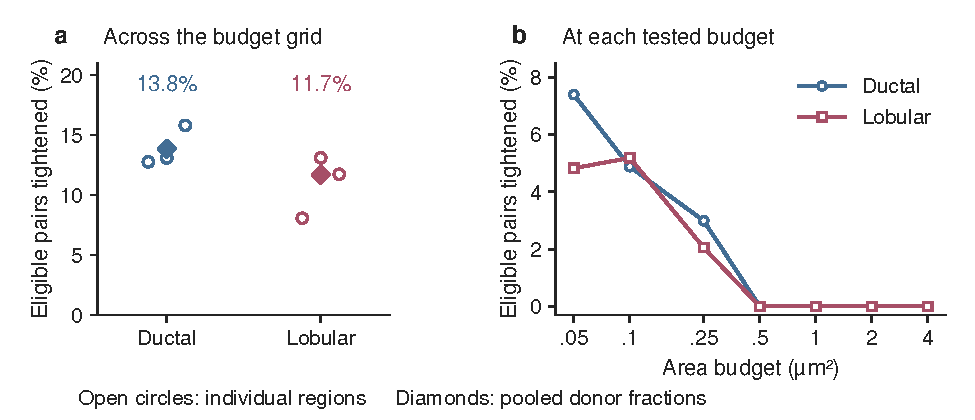
\includegraphics[width=\textwidth]{figures/donor_replication.pdf}
\caption{Replication in two breast cancer donors under the unchanged primary atlas. (a) Fractions tightened at any tested budget, by region and pooled within donor. (b) Fractions at each positive budget; lines connect tested values. Both panels use pairs whose outer width reaches two anywhere on the eight-budget grid. Pooled denominators are 1,271 ductal and 829 lobular pairs; regional denominators vary.}\label{fig:donors}
\end{figure}

\FloatBarrier

\subsection{Budget-dependent variation and saturation}\label{sec:saturation}
The primary support cap $B\le4$ and pixel pitch $p\simeq0.2125\,\mu\mathrm m$ imply a maximum paired-coordinate displacement of
\begin{equation}
 \|\Psi(t,h)-\Psi(t,0)\|_2\le\frac{3pB}{4\sqrt2}\le0.4508\,\mu\mathrm m.\label{eq:cap}
\end{equation}
Nuclear and endpoint constraints may restrict this displacement further. From budget $0.25\,\mu\mathrm m^2$ onward, the numbers of non-singleton intervals stay at 524 in lung and 5,259 in breast. Their widths can still change: 61 breast intervals widen between $0.25$ and $0.5\,\mu\mathrm m^2$, and three more between $0.5$ and $1\,\mu\mathrm m^2$. The last endpoint changes occur at about $0.24\,\mu\mathrm m^2$ in lung and $0.57\,\mu\mathrm m^2$ in breast. Thus counting only how many intervals are non-singleton would miss part of the budget's effect (Supplement~\S6).

\subsection{Wider ribbons: reach versus coverage}\label{sec:reach}
To examine larger boundary movements, we fixed support halfwidths $r=0.5,1,2,3\,\mu\mathrm m$ and 17 area budgets from 0 to 16 before computing outcomes. The paths, ordering, nuclear owners, seams and slope remain fixed. Each run requires chart halfwidth $B=\lfloor4\sqrt2r/p\rfloor/4$, with no narrower fallback. The resulting atlases satisfy the same chart and gluing construction, isolating the effect of wider supports.

At $3\,\mu\mathrm m$ support, a boundary can move up to about $2.23\,\mu\mathrm m$, but coverage falls to 16.9\% in lung and 17.8\% in breast. Wider ribbons are more often rejected because they meet a third cell or overlap another ribbon. Where they fit, they admit more count changes: a single gene has up to 17 molecules in a ribbon, and the last endpoint changes occur at about $4.9$ and $13.8\,\mu\mathrm m^2$, respectively (Supplement~\S7). The primary atlas retains narrower ribbons where needed; the fixed-width study requires the chosen width throughout.


\FloatBarrier
\subsection{Reach of independent reference assignments}
The image-only reference assigns RNA to the nearest labelled nuclear pixel within $5\,\mu\mathrm m$, or to background, excluding a five-micrometre crop-edge strip. We also use one Proseg 3.2.0 run per lung crop~\cite{proseg}, with factorization disabled after it failed on the smaller crop (Supplement~\S8). Proseg assigns 43.0\% and 90.1\% of returned molecules to background, testing broader reassignment than local boundary motion. In fresh, matched no-factorization runs, $800\,\mu\mathrm m$ inputs reduce the core background fractions from 42.5\% to 19.4\% and from 89.8\% to 62.1\%. These single-run comparisons show sensitivity to surrounding tissue; every complete assignment remains outside the atlas (Supplement~\S10).

Every width uses the same cell--gene pairs, excluding pairs affected by a missing RNA in any reference comparison. Allowing larger local movements alone does not improve reach: the wider uniform atlases lose too much boundary coverage (Figure~\ref{fig:reach}a).

\FloatBarrier
\subsection{Combining width alternatives}\label{sec:alternatives}
The union of the five complete atlases retains the primary family and admits the wider alternatives where they fit (Proposition~\ref{thm:union}). Proseg count reach rises from 6.6\% to 11.3\%, and nuclear-reference reach rises to 26.8\% in both datasets (Figure~\ref{fig:reach}b). Each endpoint still comes from one complete atlas, using the same observations, reference cells and physical-area units.

\begin{figure}[!htbp]\centering
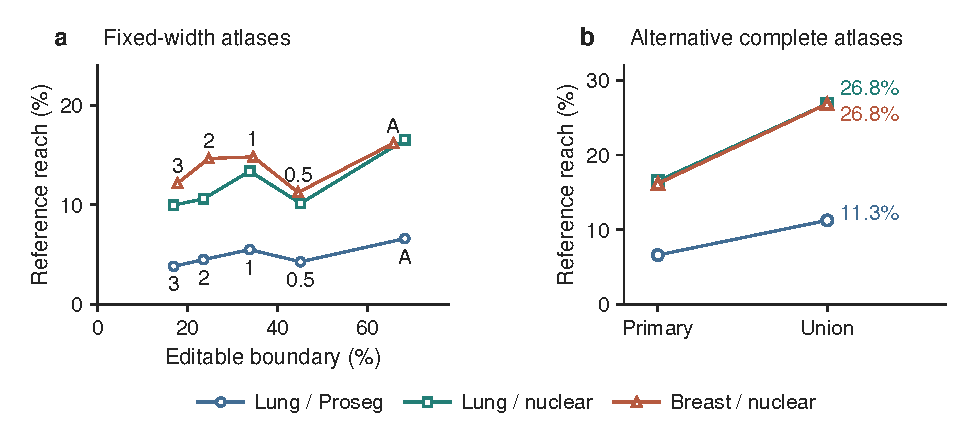
\includegraphics[width=\textwidth]{figures/reach_composite.pdf}
\caption{How ribbon choice affects reference-count reach, without an area cap. (a) Wider uniform ribbons lose editable boundary. Labels give support halfwidth in micrometres; A is the primary atlas. (b) A union retains alternatives from all five atlases. Denominators stay fixed: 2,798 changed lung Proseg counts, 1,114 lung nuclear counts and 10,965 breast nuclear counts. Proseg uses one adapted run per lung crop.}\label{fig:reach}
\end{figure}

\begin{samepage}
At $4\,\mu\mathrm m^2$, 76.4\% of the original lung counts and 65.9\% of the breast counts remain invariant across the union. Relative to the primary atlas, 298 lung and 3,595 breast intervals widen. Shared geometry also has a larger effect here: over the 17-budget grid, it tightens the independent-molecule bounds for 29 of 102 lung pairs (28.4\%) and 791 of 2,076 breast pairs (38.1\%) whose outer width reaches at least two (0.77\% and 3.11\% of all union pairs). For this comparison, we compute the independent-molecule bounds within each complete atlas and then combine their ranges, just as we combine the exact spectra (Supplement~\S5).\par
\end{samepage}

The gains reflect alternative patch selection as well as larger displacements. Coverage remains member-specific: the greatest displacement and widest boundary coverage may occur in different atlases. Each complete reference assignment remains excluded, even when some of its individual counts are attained.

\FloatBarrier
\subsection{Correctness and operating range}\label{sec:verification}
We tested the optimization and its geometric witnesses separately. Independent implementations recovered every primary interval and union spectrum, while direct boundary calculations verified witness counts and areas. The width study adds exhaustive scalar enumeration on a reproducibly selected sample of multi-transcript queries. These calculations test scalar ribbons and share prepared geometry; source-data and Proseg audits address the preceding transformations (Supplement~\S9). The coupled-interface result rests on the proof in Supplement~\S1, rather than these tissue experiments.

Small single-gene queries rarely require the count chain's full capacity. In a constructed family with known optima, computing all counts and checking their boundaries took about 0.5 seconds at 16 RNAs and 42 seconds at 128 (three-run medians). The larger case recovers all 129 count levels without enumerating $2^{128}$ assignments (Supplement~\S9.3).

On $400$ and $600\,\mu\mathrm m$ squares of the breast format-test data, completed stages took about 23 and 30 minutes for 1,363 and 3,171 complete cells, including witnesses. The $600\,\mu\mathrm m$ total is about 37 minutes when interrupted work is included. The first run uses the count chain; the second uses exact enumeration, with at most seven copies of a target gene per ribbon. Independent audits recovered every interval and verified witness counts and areas (Supplement~\S9.4).

\section{Discussion and availability}
GeoCert computes the least deformation area needed to obtain a given count. The LDHB example shows why transfers must be considered together: separately affordable transfers can exceed a shared budget, while several transfers can share the cost of one boundary movement.

Ribbon width remains the main geometric restriction. Increasing the area budget eventually stops changing counts within narrow ribbons; wider ribbons permit larger movements but cover less boundary. The union recovers alternatives where they fit, with each witness identifying the complete atlas it uses.

\paragraph{Scope and further work.}
The family fixes seams and uncovered boundaries while preserving topology and nuclear ownership. The effect recurs in the additional donors, but these experiments do not establish how well the permitted movements describe real segmentation errors. Assignment accuracy, downstream biological benefit and whole-slide scaling remain open. Multi-gene conclusions require joint queries because endpoints may use different partitions. Moving junctions and hard-budget optimization for coupled interfaces need further work.

\paragraph{Software and disclosure.}
Code (MIT license), inputs and results are at \url{https://github.com/arnavperam/geocert-recomb2027}. Source data retain 10x CC BY 4.0 attribution. Generative AI was used solely for software implementation, testing, and drafting.

\clearpage
\begin{thebibliography}{99}
\bibitem{baysor} V. Petukhov et al. Cell segmentation in imaging-based spatial transcriptomics. \emph{Nature Biotechnology} 40:345--354, 2022. doi:10.1038/s41587-021-01044-w.
\bibitem{proseg} D. C. Jones, A. E. Elz, A. Hadadianpour, H. Ryu, D. R. Glass, and E. W. Newell. Cell simulation as cell segmentation. \emph{Nature Methods} 22:1331--1342, 2025. doi:10.1038/s41592-025-02697-0.
\bibitem{li} K. Li, X. Wu, D. Z. Chen and M. Sonka. Optimal surface segmentation in volumetric images---a graph-theoretic approach. \emph{IEEE TPAMI} 28(1):119--134, 2006. doi:10.1109/TPAMI.2006.19.
\bibitem{shah} A. Shah, M. D. Abr\`amoff and X. Wu. Optimal surface segmentation with convex priors in irregularly sampled space. \emph{Medical Image Analysis} 54:63--75, 2019. doi:10.1016/j.media.2019.02.004.
\bibitem{mcshane} E. J. McShane. Extension of range of functions. \emph{Bulletin of the American Mathematical Society} 40(12):837--842, 1934. doi:10.1090/S0002-9904-1934-05978-0.
\bibitem{whitney} H. Whitney. Analytic extensions of differentiable functions defined in closed sets. \emph{Transactions of the American Mathematical Society} 36(1):63--89, 1934. doi:10.2307/1989708.
\bibitem{kz} V. Kolmogorov and R. Zabih. What energy functions can be minimized via graph cuts? \emph{IEEE TPAMI} 26(2):147--159, 2004. doi:10.1109/TPAMI.2004.1262177.
\bibitem{data} 10x Genomics. Preview Data: FFPE Human Lung Cancer with Xenium Multimodal Cell Segmentation. Xenium Onboard Analysis 2.0.0 (preview), 5 February 2024. CC BY 4.0. \url{https://www.10xgenomics.com/datasets/preview-data-ffpe-human-lung-cancer-with-xenium-multimodal-cell-segmentation-1-standard}.
\bibitem{xenium} 10x Genomics. Understanding Xenium Outputs. Xenium Onboard Analysis 2.0 documentation. \url{https://www.10xgenomics.com/support/software/xenium-onboard-analysis/2.0/analysis/xoa-output-understanding-outputs}. Accessed 31 October 2026.
\bibitem{felsner} S. Felsner and K. Knauer. Distributive lattices, polyhedra, and generalized flows. \emph{European Journal of Combinatorics} 32(1):45--59, 2011. doi:10.1016/j.ejc.2010.07.011.
\bibitem{resolvi} C. Ergen and N. Yosef. ResolVI: addressing noise and bias in spatial transcriptomics. \emph{Nature Methods} 23:2003--2014, 2026. doi:10.1038/s41592-026-03212-9.

\bibitem{hochbaum} D. S. Hochbaum. An efficient algorithm for image segmentation, Markov random fields and related problems. \emph{Journal of the ACM} 48(4):686--701, 2001. doi:10.1145/502090.502093.
\bibitem{ishikawa} H. Ishikawa. Exact optimization for Markov random fields with convex priors. \emph{IEEE TPAMI} 25(10):1333--1336, 2003. doi:10.1109/TPAMI.2003.1233908.
\bibitem{kohli} P. Kohli, L. Ladick\'y and P. H. S. Torr. Robust higher order potentials for enforcing label consistency. \emph{International Journal of Computer Vision} 82:302--324, 2009. doi:10.1007/s11263-008-0202-0.
\bibitem{zivny} S. \v{Z}ivn\'y, D. A. Cohen and P. G. Jeavons. The expressive power of binary submodular functions. \emph{Discrete Applied Mathematics} 157(15):3347--3358, 2009. doi:10.1016/j.dam.2009.07.001.
\bibitem{bidcell} X. Fu et al. BIDCell: Biologically-informed self-supervised learning for segmentation of subcellular spatial transcriptomics data. \emph{Nature Communications} 15:509, 2024. doi:10.1038/s41467-023-44560-w.
\bibitem{segger} E. Heidari, A. Moorman et al. Segger: Fast and accurate cell segmentation of imaging-based spatial transcriptomics data. \emph{bioRxiv}, 2025. doi:10.1101/2025.03.14.643160.
\bibitem{ovrlpy} S. Tiesmeyer et al. Identifying 3D signal overlaps in spatial transcriptomics data with ovrlpy. \emph{Nature Biotechnology}, published online 10 February 2026. doi:10.1038/s41587-026-03004-8.

\bibitem{bentley} J. L. Bentley and T. A. Ottmann. Algorithms for reporting and counting geometric intersections. \emph{IEEE Transactions on Computers} C-28(9):643--647, 1979. doi:10.1109/TC.1979.1675432.

\bibitem{tissue} E. D. Sun, R. Ma, P. Navarro Negredo, A. Brunet and J. Zou. TISSUE: uncertainty-calibrated prediction of single-cell spatial transcriptomics improves downstream analyses. \emph{Nature Methods} 21:444--454, 2024. doi:10.1038/s41592-024-02184-y.
\bibitem{joksch} H. C. Joksch. The shortest route problem with constraints. \emph{Journal of Mathematical Analysis and Applications} 14(2):191--197, 1966. doi:10.1016/0022-247X(66)90020-5.
\bibitem{breasttest} 10x Genomics. Example Xenium Datasets: Xenium Human Breast Gene Expression (Multimodal), two-FOV test dataset (\nolinkurl{Xenium_V1_human_Breast_2fov}). Xenium Onboard Analysis 2.0. CC BY 4.0. \url{https://www.10xgenomics.com/support/software/xenium-onboard-analysis/2.0/resources/xenium-example-data}. Accessed 31 October 2026.
\bibitem{biologicalbreast} 10x Genomics. FFPE Human Breast with Pre-designed Panel. Xenium Onboard Analysis 1.0.2; ductal and lobular carcinoma donors. CC BY 4.0. \url{https://www.10xgenomics.com/datasets/ffpe-human-breast-with-pre-designed-panel-1-standard}. Accessed 31 October 2026.
\end{thebibliography}

\end{document}
